\chapter{磁场}\label{chapter-magnetic-field}

\section{磁场}
我们在初中学过,把一根磁铁放在另一根磁铁的附近,两根磁铁的磁极之间会产生相互作用的磁力:同名磁极互相推斥,异名磁极互相吸引.我们知道,两个电荷之间相互作用的电力,不是在电荷之间直接发生的,而是通过电场传递的.同样,磁极之间相互作用的磁力,也不是在磁极之间直接发生的,而是通过磁场传递的.磁极在周围的空间里产生磁场,磁场对处在它里面的磁极有磁场力的作用.

磁铁并不是磁场的唯一来源.
1820年丹麦物理学家奥斯特($1777 \sim 1851$)做过下面的实验:把一条导线平行地放在磁针的上方,给导线通电,磁针就发生偏转(图~\ref{fig_C_1-1}).
这说明不仅磁铁能产生磁场,电流也能产生磁场,电和磁是有密切联系的.
\begin{figure}[htbp]
    \centering
    \begin{minipage}[t]{0.48\textwidth}
        \centering
        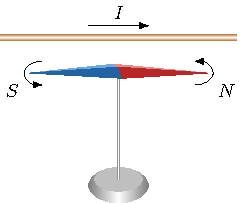
\includegraphics{fig/C/1-1.pdf}
        \caption{奥斯特实验}\label{fig_C_1-1}
    \end{minipage}
    \begin{minipage}[t]{0.48\textwidth}
        \centering
        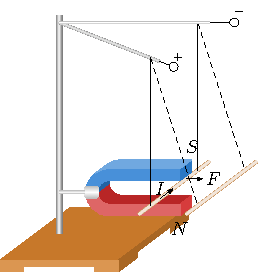
\includegraphics{fig/C/1-2.pdf}
        \caption{磁场对电流发生作用}\label{fig_C_1-2}
    \end{minipage}
\end{figure}

电流能产生磁场,反过来,磁场会不会对电流产生磁场力的作用呢?我们在初中做过的图~\ref{fig_C_1-2} 所示的实验回答了这个问题.把一段直导线放在磁铁的磁场里,当导线中通过电流时,可以看到导线因受力而发生运动.
这个实验使我们进一步知道电和磁的联系,磁场不仅对磁极产生磁场力的作用,对电流也产生磁场力的作用.
这是一个重要实验,后面我们常要提到它.

\begin{figure}[htbp]
    \centering
    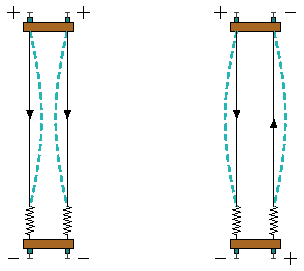
\includegraphics{fig/C/1-3.pdf}
    \caption{电流之间通过磁场发生相互作用}\label{fig_C_1-3}
\end{figure}

实验表明:电流和电流之间也会通过磁场发生相互作用.图~\ref{fig_C_1-3} 是两条平行的直导线,当通以相同方向的电流时,它们相互吸引;当通以相反方向的电流时,它们相互推斥.
这时每个电流都处在另一个电流产生的磁场里,因而受到磁场力的作用.
这就是说,电流和电流之间,就像磁极和磁极之间一样,也要通过磁场而发生相互作用.

磁场跟电场一样,是一种物质.
磁极或电流在自己周围
的空间里会产生磁场,而磁场的基本特性就是对处在它里面的磁极或电流有磁场力的作用.
这样,我们对磁极和磁极之间、磁极和电流之间、电流和电流之间的相互作用获得了统一的认识,所有这些相互作用都是通过同一种场——磁场来传递的.

\section{磁场的方向~~磁力线}
把小磁针放在磁极或电流磁场中的任一点,我们看到小磁针因受磁场力的作用,它的两极静止时不再指向南北方向,而指向一个别的方向.
在磁场中的不同点,小磁针静止时指的方向一般并不相同.
这个事实说明,磁场是有方向性的.
我们规定,在磁场中的任一点,小磁针北极受力的方向,亦即小磁针静止时北极所指的方向,就是那一点的磁场方向.

正像在电场中可以利用电力线来形象地描写各点的电场方向一样,在磁场中可以利用磁力线来形象地描写各点的磁场方向.
所谓磁力线,是在磁场中画出的一些有方向的曲线,在这些曲线上,每一点的切线方向都跟该点的磁场方向一致(图~\ref{fig_C_1-4}).
\begin{figure}[htbp]
    \centering
    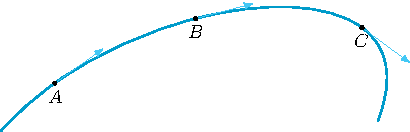
\includegraphics{fig/C/1-4.pdf}
    \caption{磁力线}\label{fig_C_1-4}
\end{figure}

实验上常用铁屑在磁场中被磁化的性质,来显示磁力线的形状.
在磁场中放一块玻璃板,在玻璃板上均匀地撒一层细铁屑,细铁屑在磁场里被磁化成“小磁针”.
轻敲玻璃板使
铁屑能在磁场作用下转动,铁屑静止时有规则地排列起来,就
显示出磁力线的形状.



图~\ref{fig_C_1-5} 是条形磁铁和蹄形磁铁的磁力线分布情况.
磁铁外部的磁力线是从磁铁的北极出来,进入磁铁的南极.


\begin{figure}[htbp]
	\centering
	\begin{subfigure}{0.4\linewidth}
		\centering
		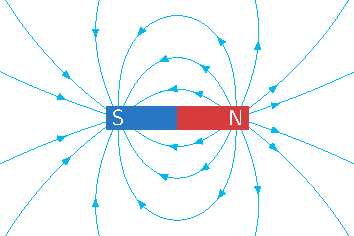
\includegraphics{fig/C/1-5a.pdf}
		\caption{条形磁铁}\label{fig_C_1-5a}
	\end{subfigure}
	\hfil
	\begin{subfigure}{0.4\linewidth}
		\centering
		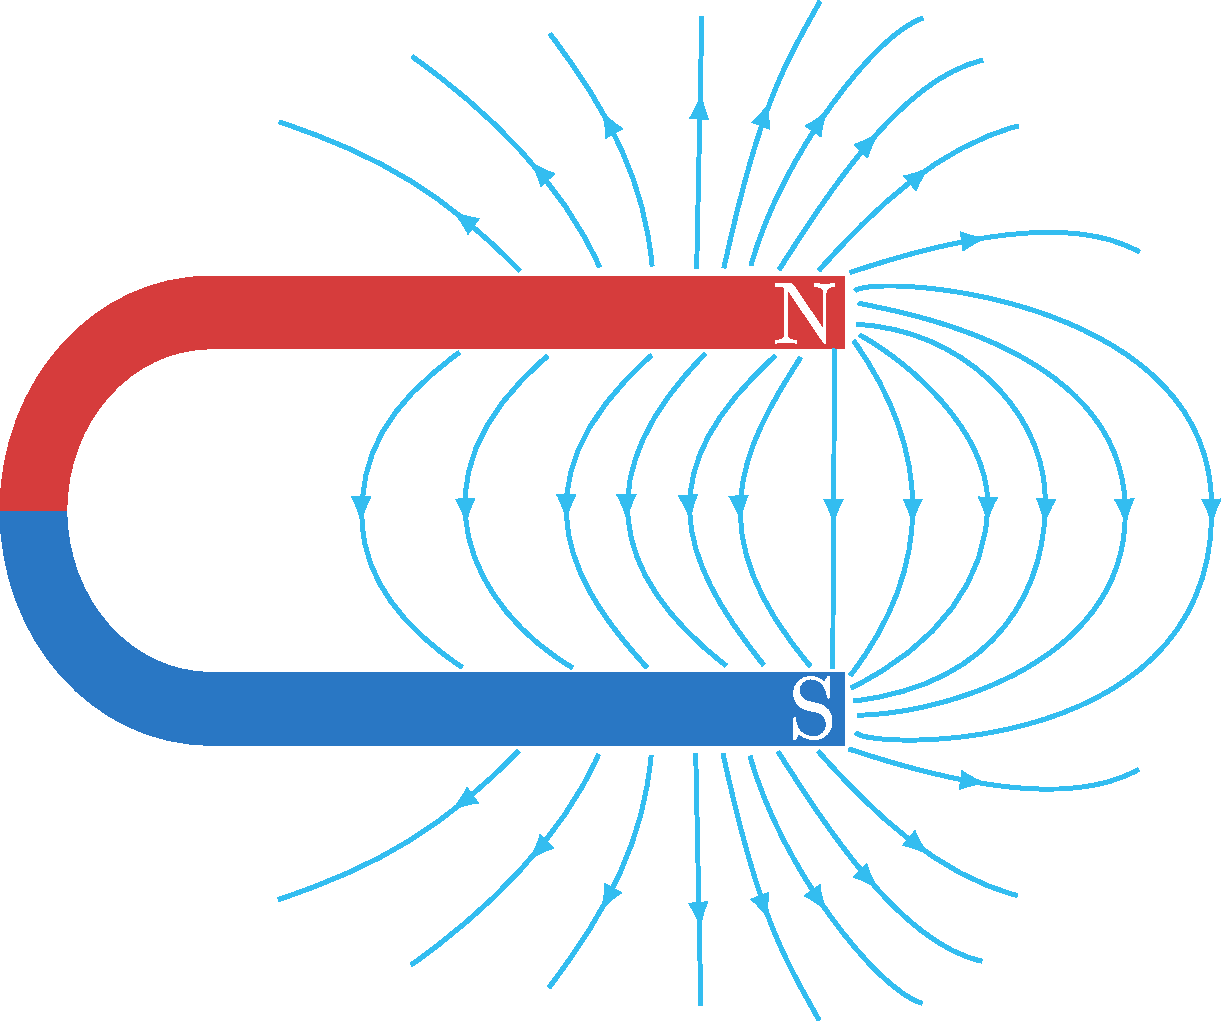
\includegraphics[height=4.3cm]{fig/C/1-5b.pdf}
		\caption{蹄形磁铁}\label{fig_C_1-5b}
	\end{subfigure}
	\caption{磁铁磁场的磁力线分布}\label{fig_C_1-5}
\end{figure}





图~\ref{fig_C_1-6} 是直线电流的磁场.直线电流磁场的磁力线,是
一些以导线上各点为圆心的同心圆,这些同心圆都在跟导线垂直的平面上.
实验表明,改变电流的方向,各点的磁场方向都变成相反的方向,即磁力线的方向随着改变.直线电流的方向跟它的磁力线方向之间的关系可以用\textbf{安培定则}(也叫\textbf{右手螺旋定则})来判定:用右手握住导线,让伸直的大拇指所指的方向跟电流的方向一致,弯曲的四指所指的方向就是磁力线的环绕方向.

\begin{figure}[htbp]
	\centering
	\begin{subfigure}{0.4\linewidth}
		\centering
		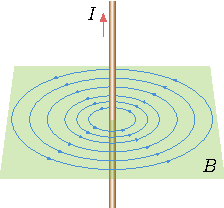
\includegraphics{fig/C/1-6a.pdf}
		\caption{磁力线分布}\label{fig_C_1-6a}
	\end{subfigure}
	\hfil
	\begin{subfigure}{0.4\linewidth}
		\centering
		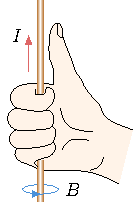
\includegraphics{fig/C/1-6b.pdf}
		\caption{安培定则}\label{fig_C_1-6b}
	\end{subfigure}
	\caption{直线电流的磁场}\label{fig_C_1-6}
\end{figure}




图~\ref{fig_C_1-7} 是环形电流的磁场.
环形电流磁场的磁力线,是
一些围绕环形导线的闭合曲线.在环形导线的中心轴线上,
磁力线和环形导线的平面垂直.
环形电流的方向跟它的磁力线方向之间的关系,也可以用\textbf{安培定则}来判定:让右手弯曲的四指和环形电流的方向一致,伸直的大拇指所指的方向就是环形导线中心轴线上磁力线的方向.

\begin{figure}[htbp]
	\centering
	\begin{subfigure}{0.4\linewidth}
		\centering
		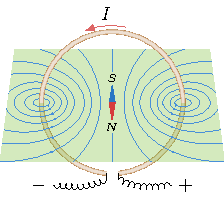
\includegraphics{fig/C/1-7a.pdf}
		\caption{磁力线分布}\label{fig_C_1-7a}
	\end{subfigure}
	\hfil
	\begin{subfigure}{0.4\linewidth}
		\centering
		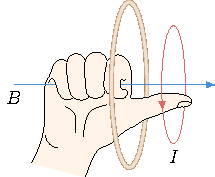
\includegraphics{fig/C/1-7b.pdf}
		\caption{安培定则}\label{fig_C_1-7b}
	\end{subfigure}
	\caption{环形电流的磁场}\label{fig_C_1-7}
\end{figure}




图~\ref{fig_C_1-8} 是通电螺线管的磁场.螺线管通电以后表现出来的磁性,很像是一根条形磁铁,一端相当于北极,另一端相当
于南极.改变电流的方向,它的南北极就对调.
通电螺线管外部的磁力线和条形磁铁外部的磁力线相似,也是从北极出
来,进入南极的.
通电螺线管内部具有磁场,内部的磁力线跟螺线管的轴线平行,方向由南极指向北极,并和外部的磁力线连接,形成一些闭合曲线.
通电螺线管的电流方向跟它的磁力线方向之间的关系,也可用\textbf{安培定则}来判定:用右手握住螺线管,让弯曲的四指所指的方向跟电流的方向一致,大拇指所指的方向就是螺线管内部磁力线的方向,也就是说,大拇指指向通电螺线管的北极.

\begin{figure}[htbp]
	\centering
	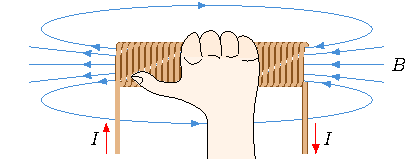
\includegraphics{fig/C/1-8.pdf}
	\caption{通电螺线管的磁场}\label{fig_C_1-8}
\end{figure}



\section{磁现象的电本质~~磁性材料}
\subsection{磁现象的电本质}


磁极和电流同样能够产生磁场,磁场对磁极和电流同样有磁场力的作用.通电螺线管和条形磁铁又那么相似.
这些现象使我们想到:磁极的磁场和电流的磁场是不是有相同的起源?这个问题现在已经有了明确的回答.
这个相同的起源就是电荷的运动.

导体中的电流是由电荷的运动形成的,因而我们不难理解通电导线的磁场是由电荷的运动产生的.那么,能不能进一步用实验直接证实:原来静止的电荷,当它运动起来的时
候就会产生磁场呢?这个问题早在一百多年以前就提出来了.1876年美国的罗兰用实验证实了这一点.
罗兰把大量的电荷加在一个橡胶圆盘上,然后使盘绕中心轴高速转动,在盘的附近用小磁针来检验运动电荷产生的磁场(图~\ref{fig_C_1-9}).
结果他发现:当带电盘转动时,小磁针果然发生了偏转,而且改变盘的转动方向或者改变所带电荷的正负时,小磁针的偏转方向也改变,磁针的偏转方向跟运动电荷所形成的电流方向间的关系同样符合安培定则.这个实验证明了运动电荷确实产生磁场,进一步揭示了磁现象的电本质.

\begin{figure}[htbp]
    \centering
    \begin{minipage}[t]{0.48\textwidth}
    	\centering
        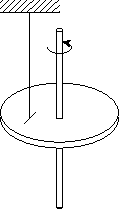
\includegraphics{fig/C/1-9.pdf}
        \caption{罗兰实验的示意图}\label{fig_C_1-9}
    \end{minipage}
    \begin{minipage}[t]{0.48\textwidth}
        \centering
        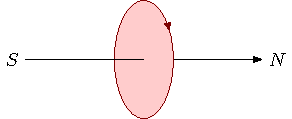
\includegraphics{fig/C/1-10.pdf}
        \caption{}\label{fig_C_1-10}
    \end{minipage}
\end{figure}


磁铁的磁场是否也是由电荷的运动产生的呢?法国科学家安培($1775 \sim 1836$),从奥斯特实验得到启示,提出了著名的分子电流的假说.他认为:在原子、分子等物质微粒内部存
在着一种环形电流,叫做分子电流,分子电流使每一个物质微粒都成为一个微小的磁体,它的两侧相当于两个磁极(图~\ref{fig_C_1-10}),这两个磁极跟分子电流不可分割地联系在一起.


安培的假说能够解释各种磁现象.
一根软铁棒,在未被磁化的时候,内部各分子电流的取向是杂乱无章的(图~\ref{fig_C_1-11a}),它们的磁场互相抵消,对外界不显磁性.
当软铁棒受到外界磁场的作用时,各分子电流的取向变得大致相同(图~\ref{fig_C_1-11b}),软铁棒就被磁化了,两端对外界显示出较强的磁作用,形成磁极.

\begin{figure}[htbp]
    \centering
    \begin{subfigure}{0.4\linewidth}
        \centering
        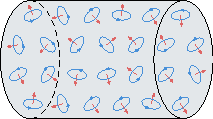
\includegraphics{fig/C/1-11a.pdf}
        \caption{}\label{fig_C_1-11a}
    \end{subfigure}
    \hfil
    \begin{subfigure}{0.4\linewidth}
        \centering
        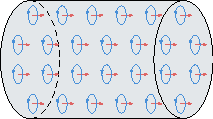
\includegraphics{fig/C/1-11b.pdf}
        \caption{}\label{fig_C_1-11b}
    \end{subfigure}
    \caption{}\label{fig_C_1-11}
\end{figure}

磁体受到高温或猛烈的敲击会失去磁性.
这是因为在激烈的热运动或机械运动的影响下,分子电流的取向又变得杂乱了.

在安培所处的时代,人们对物质内部为什么会有分子电流还不清楚.
直到二十世纪初,人类了解了原子的结构,才知道分子电流是由原子内部电子的运动形成的.
这样看来磁极的磁场和电流的磁场,它们的来源相同,都来源于电荷的运动.

\textit{运动的电荷(电流)产生磁场,磁场对运动的电荷(电流)有磁场力的作用.所有的磁现象都可以归结为运动电荷(电流)之间通过磁场而发生的相互作用}.
这就是磁现象的电本质.

\subsection{磁性材料}

实验表明,任何物质在磁场中都能够或多或少地被磁化,只是磁化的程度不同.
像铁、钴、镍那样能够被强烈磁化的物质,叫做铁磁性材料.
磁化后的铁磁性物质,它们的磁性并不因外磁场的消失而完全消失,仍然剩余一部分磁性,叫做剩磁.

铁磁性物质按剩磁的情形分为软磁性材料和硬磁性材料.
软磁性材料的剩磁弱,而且容易退磁.
软磁性材料适用于需要反复磁化的场合,可以用来制造变压器、交流发电机、电磁铁和各种高频电磁元件的铁芯.
软铁、硅钢、坡莫合金(镍铁合金)等是软磁性材料.
硬磁性材料的剩磁强,而且不易退磁,适合于制成永久磁铁,应用在磁电式仪表、扬声器、话筒、永磁电机等电器设备中.
常见的金属硬磁性材料有碳钢、钨钢、铝镍钴的合金等.

还有一种磁性材料,叫做铁氧体,它是由氧化铁和二价金属(如$ \rm{Ni} $,$ \rm{Co} $,$ \rm{Mn} $,$ \rm{Mg} $等)的氧化物组成的,在电性能上与半导体相似,在磁性上与铁磁性材料相似.
铁氧体在电子技术中已经成为不可缺少的磁性材料.在电子计算机中利用铁氧体作记忆元件.
在电子线路中广泛利用铁氧体作电感线圈的磁心.

\subsection*{练习一}
\begin{enumerate}
    \item 磁体的北极在磁场中所受的磁场力跟磁场方向同向,南极所受的磁场力跟磁场方向反向.图~\ref{fig_C_1-12} 是放在磁场中的小磁针.
    试根据小磁针所受的力说明,它将怎样转动以及静止在哪个方向.
\begin{figure}[htbp]
    \centering
    \begin{minipage}[t]{0.48\textwidth}
        \centering
        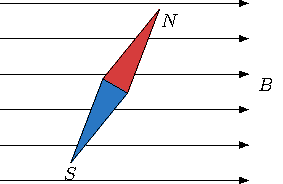
\includegraphics{fig/C/1-12.pdf}
        \caption{}\label{fig_C_1-12}
    \end{minipage}
    \begin{minipage}[t]{0.48\textwidth}
        \centering
        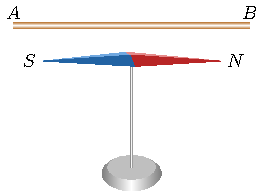
\includegraphics{fig/C/1-13.pdf}
        \caption{}\label{fig_C_1-13}
    \end{minipage}
\end{figure}
    \item 在图~\ref{fig_C_1-13} 中,当电流通过导线时,导线下面的磁针北极转向读者.试判断AB中电流的方向.
    \item 在图~\ref{fig_C_1-14} 中,当电流通过线圈时,磁针的南极指向读者.试确定线圈中电流的方向.
\begin{figure}[htbp]
    \centering
    \begin{minipage}[t]{0.48\textwidth}
        \centering
        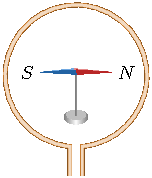
\includegraphics{fig/C/1-14.pdf}
        \caption{}\label{fig_C_1-14}
    \end{minipage}
    \begin{minipage}[t]{0.48\textwidth}
        \centering
        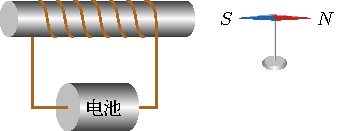
\includegraphics{fig/C/1-15.pdf}
        \caption{}\label{fig_C_1-15}
    \end{minipage}
\end{figure}

    \item 试确定图~\ref{fig_C_1-15} 中电源的正极和负板.
    \item 离开你向前运动的质子流产生的磁场是怎样的?向着你运动的电子流产生的磁场又是怎样的?
\end{enumerate}

\section{磁感应强度}
磁场不仅有方向性,而且有强弱的不同.
巨大的电磁铁能够吸起成吨的钢铁,小的磁铁只能吸起小铁钉.
我们怎样来表示磁场的强弱呢?

电场的基本特性是对其中的电荷有电场力的作用,研究电场强弱的时候,我们从分析电荷在电场中的受力情况着手,得出电场强度这个物理量来表示电场的强弱.
磁场的基本特性是对其中的电流有磁场力的作用,研究磁场的强弱,我们可以从分析电流在磁场中的受力情况着手,找出表示磁场的强弱的物理量.
为此,我们需要把一小段通电导线放在磁场中的某处,来研究它的受力情况.

把一小段通电导线放在磁场中的某处,我们发现,当导线方向跟该处的磁场方向一致时,通电导线所受的力最小,等于
零.当导线方向跟该处的磁场方向垂直时,所受的力最大.
当导线方向跟磁场方向斜交时,所受的力介于零和最大值之间.下面,为了确定起见,我们总是把一小段通电导线垂直放入磁场,也就是放在与该处磁场方向垂直的方向上.

垂直放入磁场的通电导线所受的磁场力不仅跟其中的电流强度有关,而且跟导线的长短有关.如图~\ref{fig_C_1-2} 那样,把一段通电导线垂直地放入磁场中.
实验指出:导线长度一定时,电流强度$I$越大,导线受到的磁场力$F$也越大;电流强度一定时,导线$\ell$越长,导线受到的磁场力$F$也越大.精确的实验表明:通电导线受到的磁场力$F$跟通过的电流强度$I$和导线的长度$\ell$成正比,或者说,$F$跟乘积$I\ell$成正比.
这就是说,把通电导线垂直放入磁场中的某处,无论怎样改变电流强度$I$和
导线长度$\ell$,乘积$I\ell$增大多少倍,$F$也增大多少倍.
比值$F/I\ell$跟乘积$I\ell$无关,是一个恒量.
在磁场中不同的地方,这个比值可以是不同的值.
这个比值越大的地方,表示一定长度的通电导线受到的磁场力越大,即那里的磁场越强.
因此我们可以用这个比值来表示磁场的强弱.

\textit{在磁场中垂直于磁场方向的通电导线,所受的磁场力$F$跟电流强度$I$和导线长度$\ell$的乘积$I\ell$的比值叫做通电导线所在处的\textbf{磁感应强度}}\footnote{这个物理量所以叫做磁感应强度,而没有叫做磁场强度,是由于历史上磁场强度一词已用来表示另外一个物理量.}.如果用$B$表示磁感应强度,那么,
\[B=\frac{F}{I\ell}\]

磁感应强度是一个矢量,它的大小如上式所示,它的方向
就是该点的磁场方向.

磁感应强度$B$的单位由$F$、$I$和$\ell$的单位决定.
在国际单位制中,磁感应强度的单位是\textbf{特斯拉},简称特,国际符号是$ \UTA $.1米长的导线,通过1安的电流,受到的磁场力为1牛时,磁感应强度就是1特.
\[1\UT =1 \Uspace \frac{\UNA}{\UAmA}\]

一般永磁铁的磁极附近的磁感应强度大约是$0.4 \sim 0.7$特,在电机和变压器的铁芯中,磁感应强度可达$0.8 \sim 1.4$特,通过超导材料的强电流的磁感应强度可高达1000特,而地面附近地磁场的磁感应强度大约只有$0.5\times 10^{-4}$特.

正像用电力线的疏密程度可以形象地表示电场强度的大小一样,用磁力线的疏密程度也可以形象地表示磁感应强度的大小.
在磁感应强度大的地方磁力线密一些,在磁感应强度小的地方磁力线稀一些.

如果在磁场的某一区域里,磁感应强度的大小和方向都相同,这个区域就叫做\textbf{匀强磁场}.
匀强磁场的磁力线,方向相同,疏密程度也一样,是一些分布均匀的平行直线.

匀强磁场是最简单但又是很重要的磁场,在电磁仪器和科学实验中常常要用到它.
通电长螺线管内部的磁场,距离相当近的两个平行的异名磁极间的磁场,都是匀强磁场(图~\ref{fig_C_1-16}).

\begin{figure}[htbp]
    \centering
    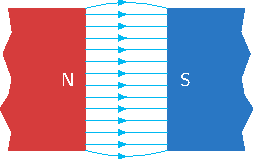
\includegraphics{fig/C/1-16.pdf}
    \caption{永磁铁间的匀强磁场}\label{fig_C_1-16}
\end{figure}

\section{磁通量}
在电学和电工学里常常要讨论穿过某一个面的磁场.为此需要引入一个新的物理量——磁通量,在下一章里就要用到它.
设在匀强磁场中有一个与磁场方向垂直的平面(图~\ref{fig_C_1-17}),磁场的磁感应强度为$B$,平面的面积为$S$.我们定义\textit{磁感应强度$B$与面积$S$的乘积,叫做穿过这个面的\textbf{磁通量}}(简称磁通).
如果用$\phi$表示磁通量,那么
\[\phi=BS \]

磁通量的意义也可以用磁力线形象地加以说明.
我们知道,磁力线越密的地方,也就是穿过单位面积的磁力线条数越多的地方,磁感应强度$B$越大.因此,$B$越大,$S$越大,穿过这个面的磁力线条数就越多.
磁通量所表示的就是穿过磁场中某个面的磁力线条数.

\begin{figure}[htbp]
    \centering
    \begin{minipage}[t]{0.48\textwidth}
        \centering
        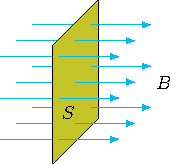
\includegraphics{fig/C/1-17.pdf}
        \caption{}\label{fig_C_1-17}
    \end{minipage}
    \begin{minipage}[t]{0.48\textwidth}
        \centering
        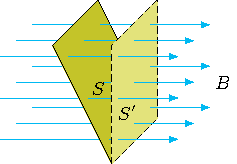
\includegraphics{fig/C/1-18.pdf}
        \caption{}\label{fig_C_1-18}
    \end{minipage}
\end{figure}


当平面$S$不跟磁场方向垂直时(图~\ref{fig_C_1-18}),穿过这个面的磁力线条数比垂直时少,因此磁通量也小.
设平面$S$在垂直于磁力线方向上的投影为$S_n$.
从图中可以看出,穿过平面$S$
的磁力线条数等于穿过投影平面$S_n$的磁力线条数.
所以穿过平面$S$的磁通量
\[\phi=BS_n=BS\cos\theta\]
如果平面跟磁场方向平行,则没有磁力线穿过这个面,这时$\theta=90^\circ$,$\cos\theta=0$,穿过这个面的磁通量为零.

在国际单位制中,磁通量的单位是\textbf{韦伯},简称韦,国际符号是$\UWbA$.在磁感应强度是1特的匀强磁场里,穿过跟磁场方向垂直的面积是1$\Umq$的平面的磁通量,就是1韦.
\[1 \UWb =1 \UTmq\]
引入了磁通量这个概念,反过来我们也可以把磁感应强
度看作是通过单位面积的磁通量,因此磁感应强度也常叫做\textbf{磁通密度},并且用$\UWbmqA$作单位.

\subsection*{练习二}
\begin{enumerate}
    \item 有人根据$B=F/I\ell$提出:磁场中某处的磁感应强度$B$跟磁场力$F$成正比,跟电流强度$I$和导线长度$\ell$的乘积$I\ell$成反比.这种提法有什么问题?错在哪里?
    \item 能不能用一小段通电导线在磁场中所受磁场力的方向来定义磁感应强度的方向?讨论一下这个问题.
    \item 长10厘米的导线,放入匀强磁场中,它的方向和磁场的方向垂直,导线中的电流强度是3.0安,受到的磁场力是$1.5\times10^{-3}$牛.求该处的磁感应强度.
    \item 把矩形线圈$abcd$放在匀强磁场中(图~\ref{fig_C_1-19}).
    线圈面积为$5\times10^{-2}\Umq$,磁感应强度为$2\times10^{-3} \UT$.
     \begin{enumerate}
        \item 当线圈平面与磁场方向垂直时,穿过线圈的磁通量是多少?
        \item 线圈平面从图所示的位置绕$OO'$轴转过$60^\circ$时,穿过线圈的磁通量是多少?
    \end{enumerate}
    \begin{figure}[htbp]
    	\centering
    	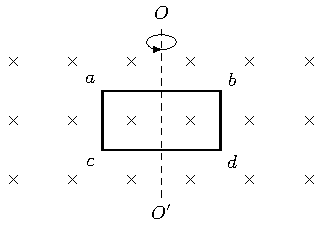
\includegraphics{fig/C/1-19.pdf}
    	\caption{}\label{fig_C_1-19}
    \end{figure}
    \item 通电螺线管内部的磁感应强度大,还是管口外部的磁感应强度大?你是根据什么判断的?
\end{enumerate}



\section{直线 电流的磁场}
前面我们已经介绍了直线电流磁场的磁力线分布(图~\ref{fig_C_1-6}),从磁力线的分布就可以知道磁场中各点的磁感应强度的方向.那么,直线电流磁场中各点的磁感应强度的大小又是怎样的呢?实验表明,磁感应强度的大小跟导线中的电流强度$I$有关系,也跟离开导线的距离$r$有关系.


如图~\ref{fig_C_1-20} 所示,在垂直于
长直导线的平面上,放一个可以自由转动的小磁针.
先让小磁针的位置不变,改变电路里的电流强度,来研究磁感应强度跟电流强度的关系.实验指出,电流强度越大,小磁针的偏转角度越大.
这说明电流强度越大,磁感应强度就越大.再让导线中的电流强度不变,改变小磁针的位置,来研究磁感应强度跟离开导线的距离的关系.实验指出,小磁针离导线越近,偏转角度越大.这说明离导线越近,磁感应强度就越大.
\begin{figure}[htbp]
	\centering
	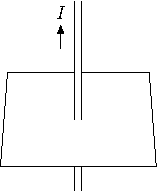
\includegraphics{fig/C/1-20.pdf}
	\caption{ }\label{fig_C_1-20}
\end{figure}


可以证明:直线电流磁场的磁感应强度$B$的大小跟电流强度$I$成正比,跟离开导线的距离$r$成反比.
写成公式就是
\[B=k\frac{I}{r}\]
其中$k$是比例恒量.

严格说来,上式只适用于无限长的直线电流.
但是实际上,当直导线的长度远大于离开导线的距离$r$时,除了导线两端附近,上式都是适用的.

环形电流磁场和通电螺线管磁场的磁感应强度的大小也可以计算出来.
它们的计算公式虽然跟直线电流不同,但有一点是相同的,即磁感应强度的大小都跟电流强度成正比.
电流强度越大,磁感应强度也越大.

\section{磁场对电流的作用力}
前而我们研究磁感应强度的时候,对电流所受的磁场力
已经作过一些讨论.
电流所受的磁场力通常叫做\textbf{安培力}.这一节讨论安培力的大小和方向.

\subsection{安培力的大小}

把一小段通电导线垂直放入磁场中,我们根据通电导线受的力$F$、导线中的电流强度$I$和导线长度$\ell$定义了磁感应强度$B=F/I\ell$.
把这个公式变形,就得到电流所受的安培力的公式:
\[F=I\ell B\]

严格说来,这个公式只适用于一小段通电导线的情形;导
线较长时,导线所在处各点的磁感应强度矢量一般并不相同,不能应用这个公式.如果磁场是匀强磁场,这个公式就适用于长的通电导线了.
\begin{figure}[htbp]
    \centering
    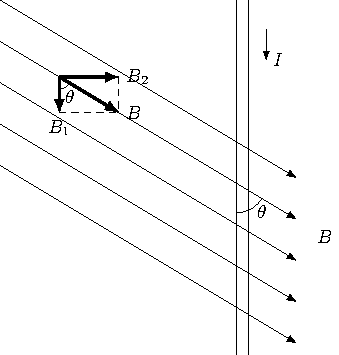
\includegraphics{fig/C/1-21.pdf}
    \caption{}\label{fig_C_1-21}
\end{figure}

如果电流方向不跟磁场方向垂直,电流受到的安培力又怎样呢?我们知道,电流方向跟磁场方向垂直时,电流受的力最大,其值可由公式$F=I\ell B$计算出;电流方向跟磁场方向平行时,电流根本不受力,即所受的力为零.
知道了电流在这两种特殊情况下所受的力,我们不难求出电流在磁场中任意方向上所受的力.如图~\ref{fig_C_1-21} 所示,当电流方向与磁场方向间有一个夹角$\theta$时,我们可以把磁
感应强度矢量$B$分解为两个分量:一个是跟电流方向平行的分量$B_1=B\cos\theta$,另一个是跟电流方向垂直的分量$B_2=B\sin\theta$.前者对电流没有作用力,电流受到的力完全是由后者决定的,即$F=I\ell B_2$.代入$B_2=B\sin\theta$,我们得到
\[F=I\ell B\sin\theta\]
这就是电流方向与磁场方向成某一角度时安培力的公式.这就是说,\textit{安培力的大小等于电流强度$I$、导线长度$\ell$、磁感应强度$B$以及$I$和$B$间的夹角$\theta$的正弦$\sin\theta$的乘积}.从上式可以看出,当$\theta =90^{\circ}$时,安培力最大,等于$I\ell B$;电流方向越偏离与磁场相垂直的方向,即$\theta$越小,安培力也越小;当$\theta =0$时,安培力最小,等于零.

在国际单位制中,上式中的各个物理量分别用牛顿、安培、米、特斯拉作单位.

\subsection{安培力的方向}


上述公式给出了安培力的大小,安培力的方向是怎样的呢?怎样判定安培力的方向,同学们在初中已经学过,这里再讨论一下.
在图~\ref{fig_C_1-2} 所示的实验中,如果把磁铁的两极调换位置来改变磁场方向,或者不改变磁场方向而改变电流方向,导线就向着相反的方向运动.
可见通电导线在磁场中的受力方向跟磁场方向,导线中的电流方向都有关系.实验表明:电流所受安培力的方向既跟磁场方向垂直,又跟电流方向垂直;也就是说,安培力的方向总是垂直于磁力线和通电导线所在的平面.

在图~\ref{fig_C_1-2} 的实验中,磁场方向跟电流方向也是垂直的,这时可以用左手定则来判定安培力的方向(图~\ref{fig_C_1-22}):伸开左手,使大拇指跟其余四个手指垂直,并且都跟手掌在一个平面内,让磁力线垂直进入手心,
并使四指指向电流方向,这时手掌所在的平面跟磁力线和导线所在的平面垂直,拇指所指的方向就是通电导线在磁场中的受力方向.
\begin{figure}[htbp]
    \centering
    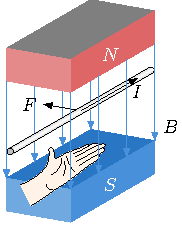
\includegraphics{fig/C/1-22.pdf}
    \caption{}\label{fig_C_1-22}
\end{figure}

我们再来看一下磁场方向不跟电流方向垂直的情形.把图~\ref{fig_C_1-2} 装置中的导线在竖直平面上转过一个角度,使磁场方向不再跟电流方向垂直,再进行观察.结果发现,导线受力的方向并没有改变,只是所受的力减小了.因此,我们仍旧可以用左手定则来判定力的方向,只是这时磁力线是倾斜进入手心的.

\section*{阅读材料:电流强度的单位——安培}
在国际单位制中,基本单位有七个,我们已经知道其中的六个,这就是:米(长度的单位),千克(质量的单位),秒(时间的单位),安培(电流强度的单位),开尔文(热力学温度的单位),摩尔(物质的量的单位).还有一个基本单位叫做坎德拉,是光学中发光强度这个物理量的单位.这个单位在中学课程中涉及不到.这里我们介绍一下安培这个单位是怎样确定的.

以前我们是用电量的单位库仑来确定安培这个单位的,似乎库仑是一个基本单位.其实在国际单位制中库仑不是基本单位,而是导出单位,安培才是基本单位.以前所以那样讲,是因为我们的知识不够,不能先讲安培这个单位.安培是利用电流之间的相互作用力来确定的,学过直线电流的磁场
和磁场对电流的作用力,现在我们有条件来介绍这个问题了.
\begin{figure}[htbp]
    \centering
    \begin{subfigure}{0.4\linewidth}
        \centering
        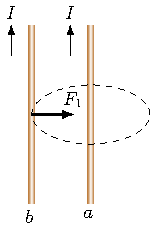
\includegraphics{fig/C/1-23a.pdf}
        \caption{}\label{fig_C_1-23a}
    \end{subfigure}
    \hfil
    \begin{subfigure}{0.4\linewidth}
        \centering
        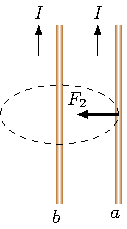
\includegraphics{fig/C/1-23b.pdf}
        \caption{}\label{fig_C_1-23b}
    \end{subfigure}
    \caption{}\label{fig_C_1-23}
\end{figure}

图~\ref{fig_C_1-23} 表示两根平行的直导线,其中通以大小和方向都相同的电流$I$.
导线$b$处于导线$a$的磁场中,因而受到这个
磁场的安培力$F_1$,从左手定则可以知道,$F_1$在纸面内自左向右,指向导线$a$,如图~\ref{fig_C_1-23a} 所示.设两导线的长度为$\ell$,两导线间的距离为$r$.
导线$a$在导线$b$处产生的磁感应强度$B=kI/r$,导线$b$所受的安培力$F_1=I\ell B=kI^2\ell/r$.同样,导线$a$处于导线$b$的磁场中,受到的安培力$F_2$在纸面内自右向左,指向导线$b$,如图~\ref{fig_C_1-23b} 所示.同样可以算出$F_2$的大小:$F_2=kI^2\ell/r$.可见两导线受到大小相等方向相反的引力,这个引力的大小$F$为
\[F=k\frac{I^2\ell}{r}\]
其中$k$是比例恒量,它的数值跟选用的单位制以及导线周围的介质有关.

在国际单位制中,安培这个单位就是利用上式来定义的.放在真空中的两根平行直导线,通以相同的稳恒电流,当两导线相距1米,每根导线在每米长度上所受的力等于$2\times10^{-7}$牛顿时,这个稳恒电流就是1安培.

根据这个定义,由上式得到
\[ 2\times10^{-7} \UN =k\frac{1 \UA^2 \times 1  \Um }{1\Um}\]
所以
\[k=2\times10^{-7}  \UNAq \]

有了安培的定义,根据公式$I=q/t$就可以定义电量的单位.
如果导线中的电流为1安培,那么每秒内通过导线横截面的电量就是1库仑.所以$1 \UC =1 \UAs $.

\subsection*{练习三}
\begin{enumerate}
    \item 图~\ref{fig_C_1-24} 表示一根放在磁场里的通电直导线.
    图中已分别标明电流、磁感应强度和安培力这三个量中两个的方向,试画出第三个量的方向.
    \begin{figure}[htbp]
        \centering
        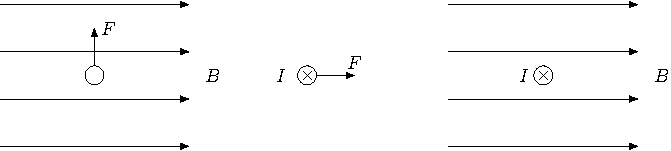
\includegraphics{fig/C/1-24.pdf}
        \caption{}\label{fig_C_1-24}
    \end{figure}
    \item 试解释为什么两根平行直导线中通以相反方向电流时,它们互相推斥.
    \item 如图~\ref{fig_C_1-25} 所示,把一根通电的直导线放在蹄形磁铁的两个磁极上方.导线可以自由移动和转动,如果电流的方向如图所示,导线将产生怎样的运动?
    \begin{figure}[htbp]
        \centering
        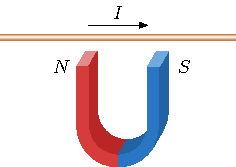
\includegraphics{fig/C/1-25.pdf}
        \caption{}\label{fig_C_1-25}
    \end{figure}
    \item 把30厘米的通电直导线放入匀强磁场中,导线中的电流强度是2.0安,磁场的磁感应强度是1.2特.求电流方向跟磁场方向垂直时导线所受的安培力.
    
    \begin{figure}[htbp]
        \centering
        \begin{minipage}[t]{0.48\textwidth}
            \centering
            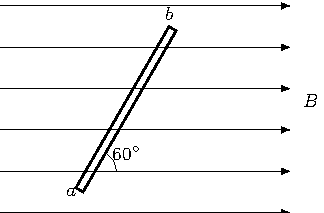
\includegraphics{fig/C/1-26.pdf}
            \caption{}\label{fig_C_1-26}
        \end{minipage}
        \begin{minipage}[t]{0.48\textwidth}
            \centering
            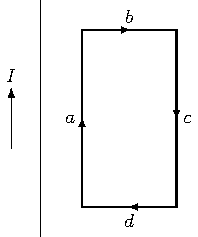
\includegraphics{fig/C/1-27.pdf}
            \caption{}\label{fig_C_1-27}
        \end{minipage}
    \end{figure}
    
    \item 在磁感应强度是$4.0\times10^{-2}$特的匀强磁场里,有一条和磁场方向相交成$60^\circ$角、长8厘米的通电直导线$ab$(图~\ref{fig_C_1-26}).通电导线$ab$所受的安培力是$1.0\times10^{-2}$牛,方向和纸面垂直指向读者.
    求导线里电流的大小和方向.
    \item 一根长2米的直导线,通有1安的电流,把它放在$B=0.2 \UT $的匀强磁场中,当导线与磁力线的夹角为$0^\circ$、$30^\circ$和$90^\circ$时,导线所受的安培力分别有多大?

    \item 如图~\ref{fig_C_1-27} 所示,在通电长导线的旁边放一个可以自由移动和转动的矩形通电线圈,线圈和导线在同一平面上,它的$a$, $c$两边和导线平行.
    试讨论一下线圈各边的受力情况,线圈在磁场中将怎样运动?
\end{enumerate}

\section{电流天平$^\star$}
应用通电导线在磁场中受力的原理,可以制成灵敏的电
流天平.用电流天平可以测出通电导线在匀强磁场中受力的大小,从而求出磁感应强度.
\begin{figure}[htbp]
    \centering
    \begin{subfigure}{0.4\linewidth}
        \centering
        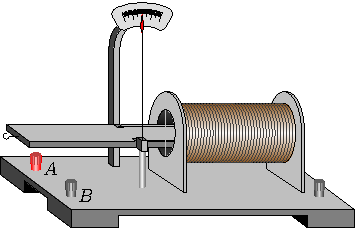
\includegraphics{fig/C/1-28a.pdf}
        \caption{}\label{fig_C_1-28a}
    \end{subfigure}
    \hfil
    \begin{subfigure}{0.4\linewidth}
        \centering
        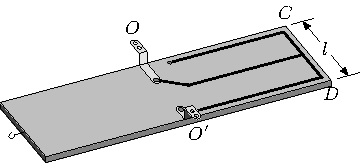
\includegraphics{fig/C/1-28b.pdf}
        \caption{}\label{fig_C_1-28b}
    \end{subfigure}
    \caption{电流天平}\label{fig_C_1-28}
\end{figure}


整个装置如图~\ref{fig_C_1-28a} 所示,它的横臂(图~\ref{fig_C_1-28b})能绕
通过点$O$和$O'$的轴自由转动.
轴的左右两侧,臂长相等.
在轴的一侧,沿着横臂的边沿固定一条U形绝缘导线.这样,
在天平的一端就有了一段短直导线$CD$,它的长度是$\ell$ \footnote{为了可以改变$\ell$的长度,仪器的U形导线中间又加了一条引线.因此,还可以用这个仪器来研究磁场对电流的作用力跟导线的长度的关系.}.天平的另一端可以悬挂砝码或细金属丝等轻小物体.调整天平,使它平衡.把有U形导线的一端放入待测的磁场中(图~\ref{fig_C_1-29}),然后给U形导线通电.
如果磁场方向和U形导线中的电流方向如图所示,$CD$段导线就受到一个向下的安培力,天平因而倾斜.
在天平的另一端加上适当的砝码,使天平恢复平衡.设待测的磁感应强度是$B$,U形导线中通过的电流强度是$I$,砝码的质量是$m$,我们就有$I\ell B=mg$,由此可求出待测的磁感应强度
\[B=\frac{mg}{I\ell}\]
\begin{figure}[htbp]
	\centering
	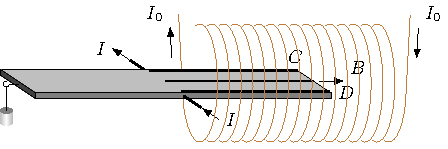
\includegraphics{fig/C/1-29.pdf}
	\caption{测定螺线管的磁感应强度}\label{fig_C_1-29}
\end{figure}

\subsection*{练习四}
\begin{enumerate}
    \item 设图~\ref{fig_C_1-29} 所示的长螺线管内部$B=1.0\times10^{-2} \UT $.
    \begin{enumerate}
        \item 与螺线管轴线平行的一条通电导线所受的力有多大?
        \item 如果$CD$的长度是2厘米,U形导线中通过的电流强度是1.0安,导线所受的力有多大?
        \item 为了使电流天平保持平衡,在另一端要加多重的砝码?
    \end{enumerate}
    \item 你自己设计一种测量磁感应强度的仪器,并说明它的原理和测定方法.
\end{enumerate}


\section{电流表的工作原理}
这一节我们讨论常用的磁电式仪表的工作原理.磁电式仪表是利用通电线圈在磁场中发生偏转的现象制成的,下面我们先讲磁场对通电线圈的作用.

\subsection{磁场对通电线圈的作用}

\begin{figure}[htbp]
    \centering
    \begin{subfigure}{0.4\linewidth}
        \centering
        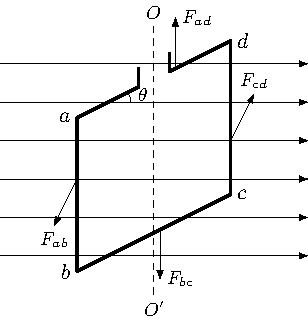
\includegraphics{fig/C/1-30a.pdf}
        \caption{}\label{fig_C_1-30a}
    \end{subfigure}
    \hfil
    \begin{subfigure}{0.4\linewidth}
        \centering
        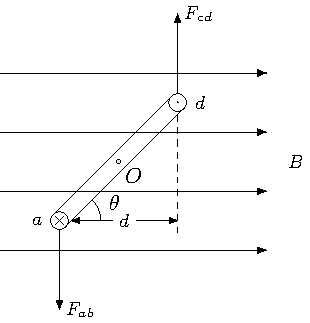
\includegraphics{fig/C/1-30b.pdf}
        \caption{}\label{fig_C_1-30b}
    \end{subfigure}
    \caption{磁场对通电线圈的作用}\label{fig_C_1-30}
\end{figure}


图~\ref{fig_C_1-30a} 表示放在匀强磁场中的通电矩形线圈,线圈平面跟磁力线成$\theta$角.线圈顶边$da$和底边$bc$所受的安培力$F_{da}$和$F_{bc}$大小相等,方向相反,彼此平衡.
$ab$和$cd$两个侧边与磁力线垂直,它们受到的安培力$F_{ab}$和$F_{cd}$虽然大小相等,方向相反,但是它们形成力偶,使线圈绕竖直轴$OO'$转动.

现在我们来求这个力偶矩.设磁感应强度为$B$,力$F_{ab}=
F_{cd}=BI·ab$,从图~\ref{fig_C_1-30b}(图~\ref{fig_C_1-30a} 的俯视图)可以看出,力偶臂$d=ad\cdot \cos\theta$,所以力偶矩$M=BI\cdot ab\cdot ad\cdot \cos\theta$,而$ab\cdot ad$等于矩形线圈的面积$S$,所以$$M=BIS\cos\theta$$

从上式可以看出,当线圈平面跟磁力线平行时,$\theta=0$,$\cos\theta=1$,所受力偶矩最大.当线圈平面跟磁力线垂直时,$\theta=90^{\circ}$,$\cos\theta=0$,力偶矩为零,这时$F_{ab}$和$F_{cd}$彼此平衡,所以线圈会停在这个位置上.

\subsection{电流表的工作原理}

常用的电流表的构造如图~\ref{fig_C_1-31} 所示.在很强的蹄形磁铁的两极间有一个固定的圆柱形铁芯,铁芯外面套一个可以绕轴转动的铝框,铝框上绕有线圈,铝框的转轴上装有两个螺旋弹簧和一个指针.线圈的两端分别接
在这两个螺旋弹簧上,被测电流就是经过这两个弹簧通入线圈的.
\begin{figure}[htbp]
    \centering
    \begin{minipage}[t]{0.48\textwidth}
        \centering
        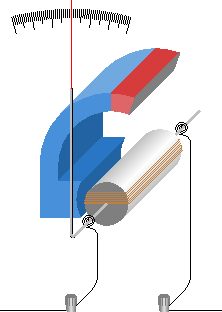
\includegraphics{fig/C/1-31.pdf}
        \caption{电流表的构造}\label{fig_C_1-31}
    \end{minipage}
    \begin{minipage}[t]{0.48\textwidth}
        \centering
        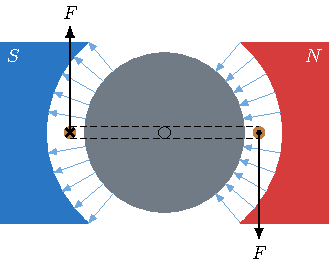
\includegraphics{fig/C/1-32.pdf}
        \caption{}\label{fig_C_1-32}
    \end{minipage}
\end{figure}


蹄形磁铁和铁芯间的磁场是均匀地辐向分布的(图~\ref{fig_C_1-32}),不管通电线圈转到什么角度,它的平面都跟磁力线平行,
因此磁场使线圈偏转的力偶矩$M_1$不随偏角而改变.另一方面,线圈的偏转使弹簧扭紧或扭松,于是弹簧产生一个阻碍线圈偏转的力矩$M_2$.线圈偏转的角度越大,弹簧的力矩$M_2$也越大.到$M_1$跟$M_2$平衡时,线圈就停在某一偏角上,固定在转轴上的指针也转过同样的偏角,指到刻度盘的某一刻度.

设电流表通电线圈的匝数为$N$,则线圈受到的力偶矩$M_1=NBIS$.由于$NBS$为定值,所以$M_1$跟电流强度$I$成正比.设$k_1=NBS$,则$M_1=k_1I$.另一方面,弹簧产生的力矩$M_2$跟偏角$\theta$成正比,即$M_2=k_2\theta$,其中$k_2$是一个比例恒量.$M_1$和$M_2$平衡时,$k_1I=k_2\theta$,即$\theta =kI$,其中$k=k_1/k_2$也是一个恒量.可见,测量时指针偏转的角度跟电流强度成正比,这就是说,这种电流计的刻度是均匀的.

这种利用永久磁铁来使通电线圈偏转的仪表叫做磁电式仪表.
这种仪表的优点是刻度均匀,准确度高,灵敏度高,可以测出很弱的电流;缺点是价格较贵,对过载很敏感,如果通入的电流超过允许值,就很容易把它烧掉,使用时要特别注意.

\subsection*{练习五}
\begin{enumerate}
    \item 如图~\ref{fig_C_1-33} 所示,把通电线圈放入永久磁铁的匀强磁场中.
    \begin{enumerate}
        \item 图~\ref{fig_C_1-33a} 中,线圈怎样转动?
        \item 图~\ref{fig_C_1-33b} 中,由上往下看线圈是顺时针转动的,磁铁哪一边是$N$极?哪一边是$S$极?
        \item 图~\ref{fig_C_1-33c} 中,由上往下看线圈是反时针转动的,画出线圈中电流的方向.
    \end{enumerate}
    \begin{figure}[htbp]
    	\centering
    	\begin{subfigure}{0.3\linewidth}
    		\centering
    		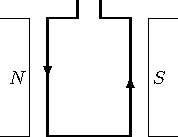
\includegraphics{fig/C/1-33a.pdf}
    		\caption{}\label{fig_C_1-33a}
    	\end{subfigure}
    	\hfil
    	\begin{subfigure}{0.3\linewidth}
    		\centering
    		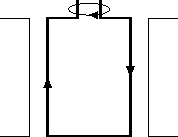
\includegraphics{fig/C/1-33b.pdf}
    		\caption{}\label{fig_C_1-33b}
    	\end{subfigure}
    	\hfil
    	\begin{subfigure}{0.3\linewidth}
    		\centering
    		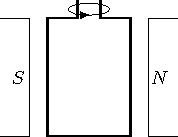
\includegraphics{fig/C/1-33c.pdf}
    		\caption{}\label{fig_C_1-33c}
    	\end{subfigure}
    	\caption{}\label{fig_C_1-33}
    \end{figure}
    \item 有一个匝数为10匝的矩形线圈,长为25厘米,宽为10厘米,放在$B=1.5\times10^{-3}\UT $的匀强磁场中,通以1.5安的电流,求它所受的最大的力偶矩.
    \item 图~\ref{fig_C_1-30} 所示的放在磁场中的线圈,当转到线圈平面跟磁力线垂直的位置时,会不会立即停在这个位置上?为什么?定性地分析一下线圈在停下来之前的运动情况.
    有什么办法可以使通电线圈不停下来而继续转动?
    \item 电流表中通以相同的电流时,指针的偏转角度越大,表示电流表的灵敏度越高.
    定性地分析一下,有哪些因素会影响磁电式电流表的灵敏度.
\end{enumerate}


\section{磁场对运动电荷的作用力}
我们知道,磁场对电流有作用力.
既然电流是电荷的运
动产生的,我们自然会想到,磁场力可能是直接作用在运动电荷上的.
作用在整个导线上的安培力,不过是作用在运动电荷上的力的宏观表现.


现在用实验来检验这个想法.图~\ref{fig_C_1-34} 是一个电子射线
管,从阴极发射出来的电子束,在阴极和阳极间的高电压作用下,轰击到荧光屏上激发出荧光,我们就可以看到电子束运动的径迹.实验表明,在没有外磁场时电子束是沿直线前进的(图~\ref{fig_C_1-34a}).
如果把射线管放在蹄形磁铁的两极间,从荧光屏上可以看到电子束运动的径迹发生了弯曲(图~\ref{fig_C_1-34b}). 这表明运动电荷确实受到了磁场的作用力,磁场对运动电荷的作用力通常叫做\textbf{洛仑兹力}.
\begin{figure}[htbp]
	\centering
	\begin{subfigure}{0.4\linewidth}
		\centering
		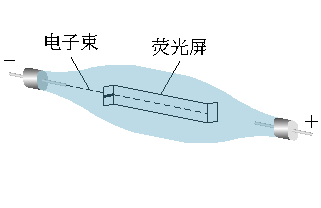
\includegraphics{fig/C/1-34a.pdf}
		\caption{}\label{fig_C_1-34a}
	\end{subfigure}
	\hfil
	\begin{subfigure}{0.4\linewidth}
		\centering
		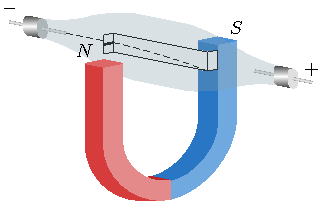
\includegraphics{fig/C/1-34b.pdf}
		\caption{}\label{fig_C_1-34b}
	\end{subfigure}
	\caption{电子束在磁场中的偏转}\label{fig_C_1-34}
\end{figure}


洛仑兹力的方向也可以用左手定则来判定:伸开左手,让磁力线进入手心,四指指向正电荷运动的方向,那么拇指所指的方向就是正电荷所受的洛仑兹力的方向.
运动的负电荷在磁场中所受的洛仑兹力,方向跟正电荷相反.

洛仑兹力的大小可以从磁场对电流的作用力计算出来.设导线中单位体积内含有的运动电荷数是$n$,每个电荷的电量是$q$,电荷的平均定向移动速率是$v$,导线的横截面积是$S$,
那么,通过导线的电流强度就是
\[I=nqvS\]

磁场对电流的作用力是$F=I\ell B\sin\theta$.这个力可以看作
是作用在每个运动电荷上的洛仑兹力的合力.设洛仑兹力为$f$,这段导线内运动电荷的总数为$N$,则$Nf=F$,即$Nf=I\ell B\sin\theta$,代入$I=nqvS$,得到
\[Nf=nqvS\ell B\sin\theta \]
导线中运动电荷总数$N$,等于单位体积内的运动电荷数$n$跟体积$S\ell$的乘积,即$N=nS\ell$,因此上式简化为
\[f=qvB\sin\theta \]
这就是说,\textit{洛仑兹力的大小等于电荷的电量$q$、电荷的速率$v$、磁感应强度$B$以及$v$和$B$间的夹角$\theta$的正弦$\sin\theta$的乘积}.在国际单位制中,上式中的各个物理量分别用牛顿、库仑、米/秒、特斯拉作单位.

当$\theta=90^{\circ}$时,即电荷的运动方向跟磁场方向垂直时,电荷所受的洛仑兹力最大,等于$qvB$.当$\theta=0$时,即电荷的运动方向跟磁场方向一致时,电荷所受的洛仑兹力最小,等于零.当$\theta$角为其他数值时,洛仑兹力的大小在最大值和最小值之间.

\subsection*{练习六}

\begin{enumerate}
    \item 如图~\ref{fig_C_1-35} 所示,带电粒子以速率$v$射入匀强磁场.分别标出带电粒子所受洛仑兹力的方向.
    \begin{figure}[htbp]
        \centering
        \begin{subfigure}{0.23\linewidth}
            \centering
            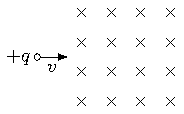
\includegraphics{fig/C/1-35a.pdf}
            \caption{}\label{fig_C_1-35a}
        \end{subfigure}
        \hfil
        \begin{subfigure}{0.23\linewidth}
            \centering
            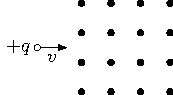
\includegraphics{fig/C/1-35b.pdf}
            \caption{}\label{fig_C_1-35b}
        \end{subfigure}
        \hfil
        \begin{subfigure}{0.23\linewidth}
            \centering
            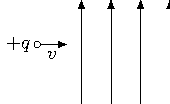
\includegraphics{fig/C/1-35c.pdf}
            \caption{}\label{fig_C_1-35c}
        \end{subfigure}
        \hfil
        \begin{subfigure}{0.23\linewidth}
            \centering
            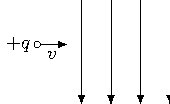
\includegraphics{fig/C/1-35d.pdf}
            \caption{}\label{fig_C_1-35d}
        \end{subfigure}
        \caption{}\label{fig_C_1-35}
    \end{figure}
    \item 一个带电粒子在空间中运动时没有发生偏转,能不能说明这个空间中没有磁场?为什么?
    \item 一个电子以速率$v$射入磁感应强度为$B$的匀强磁场中,电子沿什么方向射入,受到的洛仑兹力最大?最大值是多大?沿什么方向射入,不受洛仑兹力作用?
    \item 电子的速率$v=3.0\times10^6 \Ums$,垂直射入$B=0.1 \UT $的磁场中,它受到的洛仑兹力是多大?
    \item 一个电子以$1.2\times10^7\Ums$的速率射入磁感应强度为0.02特的匀强磁场中.当速率$v$与磁感应强度$B$的夹角$\theta$为$30^{\circ}$和$60^{\circ}$时,电子所受洛仑兹力分别是多大?
    \item 一电荷$q$在某一匀强磁场中运动,判断下面几种说法是否正确,并说明理由.
\begin{enumerate}
    \item 只要速度的大小相同,所受的洛仑兹力就相同.
    \item 如果速度不变,把电荷$q$改为$-q$,洛仑兹力的方向将反向,但大小不变.
    \item 如果速度不变,把$B$改为反向,洛仑兹力的方向将反向,但大小不变.
\end{enumerate}

\end{enumerate}


\section{带电粒子在磁场中的运动}
带电粒子在磁场中运动时受到洛仑兹力的作用,已知洛仑兹力,利用力学中学过的运动学和动力学的知识,就可以确定带电粒子在磁场中的运动情况.

现在我们研究一种简单的情形.一个带电粒子在匀强磁场中运动,它的初速度方向跟磁场方向垂直,粒子的运动轨迹将是怎样的呢?

由于初速度的方向和洛仑兹力的方向都在跟磁场方向垂直的平面内,没有任何作用使粒子离开这个平面,所以粒子只能在这个平面内运动.
洛仑兹力总是跟粒子的运动方向垂直,只改变粒子速度的方向,不改变粒子速度的大小,所以粒子的速率$v$是恒定的.这时洛仑兹力$f=qvB$的大小也是恒定的,它对运动粒子起着向心力的作用.因此粒子的运动一定是匀速圆周运动(图~\ref{fig_C_1-36}).
\begin{figure}[htbp]
    \centering
    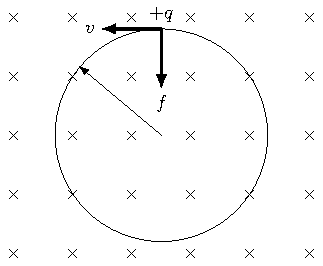
\includegraphics{fig/C/1-36.pdf}
    \caption{带电粒子的圆周运动}\label{fig_C_1-36}
\end{figure}

上述推论可以用实验来验证.
实验所用的仪器如图~\ref{fig_C_0-1} 所示,是一种特制的电子射线管,由电子枪发出的电子射线可以
使管内的低压水银蒸气(或氢气)发出辉光,显示出电子的径迹.
在暗室中可以清楚地看到:没有磁场作用时,电子的径迹是直线;在管子外面加上一个匀强磁场(这个磁场是由两个平行的通电环形线圈产生的),电子的径迹就弯曲成圆弧.
\begin{figure}[htbp]
	\centering
	\begin{subfigure}{0.46\linewidth}
		\centering
		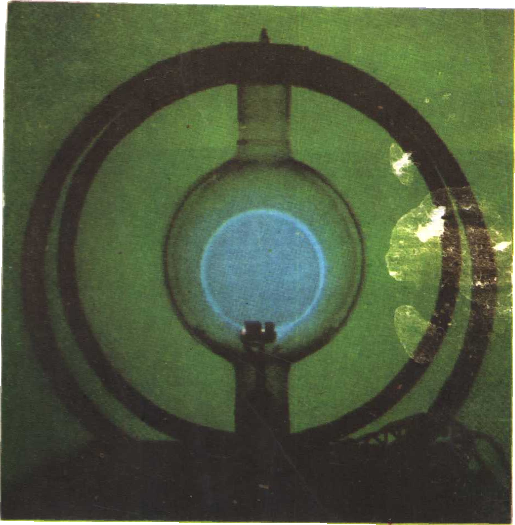
\includegraphics[height=5cm]{fig/C/0-0.pdf}
		\caption{}\label{fig_C_0-1a}
	\end{subfigure}
	\hfil
	\begin{subfigure}{0.46\linewidth}
		\centering
		\includegraphics[height=5cm]{fig/C/0-1.pdf}
		\caption{}\label{fig_C_0-1b}
	\end{subfigure}
	\caption{电子射线在磁场作用下弯成圆形}\label{fig_C_0-1}
\end{figure}


在高中二年级我们学过带电粒子在电场中的运动.
在现代科学技术中,常常要使带电粒子在电场的作用下运动,或者在磁场的作用下运动,或者在电场和磁场的共同作用下运动.例如电视机中的显像管、电子显微镜和我们将要学到的回旋加速器等,都是利用电场和磁场来控制电荷的运动的.

\begin{example}
    一个初速度为零的质子,经过电压是$1.3\times10^3$伏的电场加速后,垂直进入磁感应强度$B$是0.20特的匀强磁场中.
    试求:
    \begin{enumerate}
        \item 质子进入磁场时的速率;
        \item 质子在磁场中运动的轨道半径;
        \item 质子做匀速圆周运动的周期.
    \end{enumerate}
质子的质量$m=1.67\times10^{-27}$千克,电量$q=1.6\times10^{-19}$库.
\end{example}

\begin{solution}
    \begin{enumerate}
        \item 质子在电场中得到的动能等于电场所做的功,即$\dfrac{1}{2}mv^2=qU$.
        所以质子进入磁场时的速率
        \[\begin{split}
            v&=\sqrt{\frac{2qU}{m}}\\
            &=\frac{2\times 1.6\times 10^{-19}\times1.3\times10^3}{1.67\times 10^{-27}}\Ums\\
            &=5.0\times 10^5\Ums
        \end{split}\]
        \item 质子在磁场中做匀速圆周运动的向心力是由洛仑兹力$f=qvB$提供的,所以$qvB=mv^2/r$,解出$r$,得到
        \begin{equation}\label{eq_C_1-1}
            r=\frac{mv}{qB}
        \end{equation}
        代入数值得到
       \[\begin{split}
           r&=\frac{mv}{qB}=\frac{1.67\times 10^{-27}\times 5.0\times 10^5}{1.6\times 10^{-19}\times 0.2} \Um \\
           &=2.6\times 10^{-2} \Um 
       \end{split}\]
        
        
        \item 匀速圆周运动的周期$T=2\pi r/v$,把 \eqref{eq_C_1-1} 式代入,得到
\begin{equation}\label{eq_C_1-2}
    T=\frac{2\pi m}{qB}
\end{equation}
        代入数值得到
        \[\begin{split}
            T&=\frac{2\pi m}{qB}=\frac{2\times 3.14\times 1.67\times 10^{-27}}{1.6\times 10^{-19}\times 0.2} \Us \\
            &=3.3\times 10^{-7} \Us 
        \end{split}\]
    \end{enumerate}
\end{solution}

从 \eqref{eq_C_1-1} 式知道,带电粒子在匀强磁场中做匀速圆周运动的
轨道半径跟粒子的速率成正比,速率越大,轨道半径也越大.
从 \eqref{eq_C_1-2} 式知道,带电粒子在匀强磁场中做匀速圆周运动的周期跟轨道半径和运动速率无关.这是一个很重要的结论,我们在后面要讲到的回旋加速器就是依据这个道理制成的.
        
\subsection*{练习七}
\begin{enumerate}
    \item 电子以$1.6\times10^6\Ums$的速率垂直射入$B=10^{-4} \UT $的匀强磁场中,求电子做圆周运动的轨道半径和周期.
    \item 电子垂直射入$B=7.0\times10^{-4} \UT $的匀强磁场中,做圆周运动的轨道半径为$3.0\times10^{-2}$米,求电子运动的速率.
    \item 能量是5.3兆电子伏的$\alpha$粒子垂直进入磁感应强度是1.0特的匀强磁场中.
    试确定作用在$\alpha$粒子上的洛仑兹力和$\alpha$粒子的轨道半径.$\alpha$粒子即氦核,质量为$6.6\times10^{-27}$千克,带有两个基本电荷的正电.
    \item 具有相同动能的质子、氘核和$\alpha$粒子垂直进入同一匀强磁场.
    试比较这些粒子轨道半径的大小.
    氘核的质量为质子的两倍,带有一个基本电荷的正电.
    \item 两个电子分别以速率$v$和$2v$垂直射入匀强磁场中,经磁场偏转后,哪个电子先回到原来的出发点?
    \item 在匀强磁场中,带电粒子的运动方向不和磁感应强度的方向垂直,它的运动径迹将是什么样的曲线?(只要求定性说明)
\end{enumerate}


\section{荷质比的测定~~质谱仪}
\subsection{荷质比的测定}

带电粒子的电荷与质量之比,叫做\textbf{荷质比}.每种带电微观粒子都带有一定的电荷,具有一定的质量,所以荷质比是带电微观粒子的基本参量.

带电粒子在电场和磁场中运动时,所受的电场力和磁场力跟粒子所带的电量成正比,得到的加速度跟粒子的质量成反比,因而粒子的运动情况依赖于粒子的荷质比.这样,我们研究带电粒子在电场和磁场中的运动情况,反过来就可以确定粒子的荷质比.

图~\ref{fig_C_1-37} 是测定荷质比的一种装置.让中性的气体分子进入电离室$A$,在那里被电离成离子.这些离子从电离室的
小孔飘出,从缝$S_1$进入加速电场中被加速.然后让粒子垂直进入匀强磁场中做匀速圆周运动,最后打在照相底片$D$上.
\begin{figure}[htbp]
    \centering
    \includegraphics{fig/C/1-37.pdf}
    \caption{}\label{fig_C_1-37}
\end{figure}

设粒子所带的电量是$q$,加速电场两极间的电势差是$U$,粒子进入缝$S_1$时速度很小,接近于零,粒子离开加速电场时所获得的动能就是
\begin{equation}\label{eq_C_1-3}
\frac{1}{2}mv^2=qU    
\end{equation}

设匀强磁场的磁感应强度是$B$,粒子做匀速圆周运动的轨道半径是$r$,由于向心力是洛仑兹力提供的,所以
\begin{equation}\label{eq_C_1-4}
    \frac{mv^2}{r}=qvB
\end{equation}
由 \eqref{eq_C_1-3} 和 \eqref{eq_C_1-4} 两式中消去$v$,我们得到
\[\frac{q}{m}=\frac{2U}{B^2r^2}\]

上式右方的各物理量都可以由实验测出来,这样就可以得到粒子的荷质比.这里我们看到,微观量的大小是通过宏观量的测定而得到的.

测定荷质比,对人类认识微观粒子有重要作用.人类认
识的第一种亚原子粒子——电子,最初就是由测定它的荷质比而被发现的.十九世纪末,英国科学家汤姆生在研究阴极射线时测定了阴极射线粒子的荷质比.
他所用的方法虽然跟上述方法不同,但根据的原理也是带电粒子在电场和磁场中的偏转.
汤姆生的测定导致他发现阴极射线粒子就是电子,这个问题我们将在第\ref{chapter-atomic-structure}章讲述.

汤姆生测得的阴极射线粒子的荷质比约为$2\times10^{11}  \UCkg $,现在测得的电子荷质比的精确值是
\[\frac{e}{m}=1.7588047\times10^{11} \UCkg  \]
通常可取作$e/m=1.76\times10^{11} \UCkg $.

\subsection{质谱仪}

在图~\ref{fig_C_1-37} 所示的装置中,如果带电粒子的电量相同,而质量$m$有微小差别,它们进入磁场后将沿着不同的半径做圆周运动,打到照相底片的不同地方,在底片上形成若干谱线状的细条,叫做质谱线.每一条谱线对应于一定的质量;从谱线的位置可以知道圆周的半径$r$,已知带电粒子的电量$q$,就可以算出它的质量$m$.这种仪器叫做质谱仪,图~\ref{fig_C_1-37} 就是质谱仪的原理图.利用质谱仪对某种元素进行测量,可以准确地测出各种同位素的原子量.图中所示的是锗的质谱线,在谱线上标出的数字是锗同位素的质量数.

质谱仪最初也是由汤姆生设计的,他用质谱仪首先得到了氖20和氖22的质谱线,证实了同位素的存在.后来经过多次改进,质谱仪已成了一种十分精密的仪器,是测定带电粒子质量和分析同位素的重要工具.


\subsection*{练习八}
\begin{enumerate}
    \item 在图~\ref{fig_C_1-37} 中,设离子室$A$中产生的是钠离子,加速电压$U=705 \UV $,磁感应强度$B=3. 85\times10^{-1} \UT$,$r=5 \Ucm$,求钠离子的荷质比.
    \item 在图~\ref{fig_C_1-37} 所示的装置中,离子从小孔飘出时速度并不相同,因此经加速电场加速后,从缝$S_2$射出时速度也不相同,这对实验有一定影响.于是人们提出在缝$S_2$和$S_3$之间加一个\textbf{速度选择器}(图~\ref{fig_C_1-38}),其中$D_1$和$D_2$是两个平行金属板,分别连在电源的两极上,其间有一定的电场强度$E$;同时在这空间加有垂直于电场方向的磁场,磁感应强度为$B$.这时具有一定速度的带电粒子,从缝$S_2$垂直进入后,可以不发生偏转,由缝$S_3$射出;而具
有其他速度的带电粒子都发生偏转,不能由缝$S_3$射出.
为什么?这个一定的速度$v$有多大?
\begin{figure}[htbp]
    \centering
    \includegraphics{fig/C/1-38.pdf}
    \caption{速度选择器的原理示意图}\label{fig_C_1-38}
\end{figure}
\item 带电粒子带正电或者带负电,会不会影响速度选择器对它们的速度的选择?如果把图~\ref{fig_C_1-38} 中的电场方向改变为相反的方向,或者把磁场方向改变为相反的方向,速度选择器还能不能使用?如果把电场和磁场同时改变为相反的方向,还能不能使用?
\end{enumerate}

\section{回旋加速器}


在现代物理学中,为了研究物质的微观结构,往往要用能量很高的带电粒子去轰击各种原子核,观察它们的变化情况.例如,要从原子核中把中子或质子打出来,就得用8兆电子伏的质子.为了探索质子的内部结构,使用了200亿电子伏的电子去轰击质子.怎样才能在实验室大量产生这样高能量的带电粒子呢?这就要用一种新的实验设备——加速器.

我们已经学过,利用电场可以使带电粒子加速.早期制成的加速器,就是用高压电源的电势差来加速带电粒子的.
这种类型的加速器受到实际所能达到的电势差的限制,粒子获得的能量并不太高,只能达到几十万到几兆电子伏.
1932年美国物理学家劳仑斯发明了回旋加速器,很巧妙地克服了这个困难.
这种加速器不是利用高电压使粒子一次得到巨大的速度,而是用电压较低的高频电源,使粒子每隔一定的时间受到一次加速,经过多次加速后达到巨大的速度.

现在来看一看回旋加速器的工作原理.


图~\ref{fig_C_1-39} 表示从放在$A_0$处的粒子源发出一个带正电的粒子,它以某一速率$v_0$垂直进入匀强磁场中,在磁场中做匀速圆周运动.
经过半个周期,当它沿着半圆弧$\widering{A_0A_1}$到达$A_1$时,我们在$A_1A'_1$处造成一个向上的电场,使这个带电粒子在$A_1A_1'$处受到一次电场的加速,速率由$v_0$增加到$v_1$.然后粒子以速率$v_1$在磁场中做匀速圆周运动.
我们知道,粒子的轨道半径跟它的速率成正比,因而粒子将沿着半径增大了的圆周运动.
又经过半个周期,当它沿着半圆弧$\widering{A'_1A'_2}$到达$A'_2$时,我们在$A'_2A_2$处造成一个向下的电场,使粒子又一次受到电场的加速,速率增加到$v_2$.如此继续下去,每当粒子运动到$A_1A'_1$、$A_3A'_3$等处时都使它受到一个向上电场的加速,每当粒子运动到$A'_2A_2$、$A'_4A_4$等处时都使它受到一个向下电场的加速,这样,粒子将沿着图示的螺线$A_0A_1A'_1A'_2A_2$……回旋下去,速率将一步一步地增大.

\begin{figure}[htbp]
	\centering
	\includegraphics{fig/C/1-39.pdf}
	\caption{}\label{fig_C_1-39}
\end{figure}




我们讲过,带电粒子在匀强磁场中做匀速圆周运动的周期$T=2\pi m/qB$跟运动速率和轨道半径无关,对一定的带电粒子和一定的磁感应强度来说,这个周期是恒定的.因此,尽管粒子的速率和半径一次比一次增大,运动周期却始终不变,即粒子由$A$沿半圆弧$\widering{A_0A_1}$运动到$A_1$,由$A'_1$沿半圆弧$\widering{A'_1A'_2}$
运动到$A'_2$……经过的时间都等于半个周期,即$T/2$.
如果像图~\ref{fig_C_1-40} 所示那样,在直径$AA$、$A'A'$处造成一个交变电场,使它也
以相同的周期$T$往复变化,那就可以保证粒子每经过直径$AA$
和$A'A'$时都正好赶上适合的电场方向而被加速.这一点仔细研究一下图~\ref{fig_C_1-40} 就会明白了.

\begin{figure}[htbp]
	\centering
	\begin{subfigure}{0.4\linewidth}
		\centering
		\includegraphics{fig/C/1-40a.pdf}
		\caption{}\label{fig_C_1-40a}
	\end{subfigure}
	\hfil
	\begin{subfigure}{0.4\linewidth}
		\centering
		\includegraphics{fig/C/1-40b.pdf}
		\caption{}\label{fig_C_1-40b}
	\end{subfigure}
	\caption{左图:粒子运动到$A_1$时被电场加速.
		右图:经过半周期,粒子运动到$A'_2$,电场改变了方向,粒子又被电场加速.}\label{fig_C_1-40}
\end{figure}

回旋加速器是怎样实现上述加速粒子过程的呢?回转加速器的核心部分是两个$D$形的金属扁盒(图~\ref{fig_C_1-41}).这两个$D$形盒就像是沿着直径把一个圆形的金属扁盒切成的两半.两个$D$形盒之间留一个窄缝,在中心附近放有粒子源.$D$形盒装在真空容器中,整个装置放在巨大电磁铁的两极之间,磁场方向垂直于$D$形盒的底面.

\begin{figure}[htbp]
	\centering
	\includegraphics{fig/C/1-41.pdf}
	\caption{回旋加速器的$D$形盒}\label{fig_C_1-41}
\end{figure}


如果把两个$D$形盒分别接在频率$f=1/T=qB/(2\pi m)$的高频电源的两极上(频率的数量级为$10^6$赫),就可以在$D$形盒的窄缝中造成图~\ref{fig_C_1-40} 所示的交变电场.这样,从粒子源发出的带电粒子就可以像图~\ref{fig_C_1-39} 所示那样不断被加速.为什么
要使带电粒子在$D$形盒中运动呢?这是因为考虑到静电屏蔽作用,金属盒可以屏蔽外界电场;盒内的电场很弱,这样才能保证粒子在盒内只受磁力的作用而做匀速圆周运动.

带电粒子在$D$形盒内沿螺线轨道逐渐趋于盒的边缘,达到预期的速率后,用特殊装置把它们引出.

回旋加速器的出现,使人类在获得具有较高能量的粒子方面前进了一步.
但是,在三十年代末期已经发现,用回旋加速器加速质子,在能量达到$25 \sim 30$兆电子伏之后,就很难进一步提高了.这是因为,在粒子的能量很高的时候,它的运动
速度接近于光速,按照狭义相对论,这时粒子的质量将随着速率的增加而增大.
因此,粒子在磁场中回旋一周所需的时间要发生变化,交变电场的频率不再跟粒子运动的频率一致,这就破坏了加速器的工作条件,进一步提高粒子的速率就不可能了.

为了把带电粒子加速到更高的能量,以适应高能物理实验的需要,人们设计制造了各种类型的新型加速器,如同步加速器、电子感应加速器、直线加速器等等.
这些加速器都考虑了相对论效应,可以把带电粒子加速到几千兆电子伏以上.
目前同步加速器能够把质子加速到$10^6$兆电子伏.

\section*{复习题}
\begin{enumerate}
    \item 奥斯特用什么实验发现电流周围存在着磁场的?人们对磁极和磁极之间、磁极和电流之间、电流和电流之间的相互作用是怎样获得统一的认识的?
    \item 磁场中某一点的磁场方向是怎祥规定的?怎样用安培定则来判断直线电流、环形电流、通电螺线管的磁场方向?
    \item 安培的分子电流假说的内容是什么?什么是磁现象的电本质?
    \item 什么叫铁磁性材料?软磁性材料和硬磁性材料的性质有什么区别?各有什么用途?
    \item 什么叫磁场的磁感应强度?写出磁感应强度的定义式.磁感应强度的方向是怎样的?为什么说用磁力线可以形象地表示磁场?
    \item 什么叫磁通量?写出它的定义式.怎样用磁力线形象地说明磁通量?
    
    \item 直线电流磁场的磁感应强度跟电流强度、离开导线的距离各是什么关系?写出计算直线电流磁场的磁感应强度的公式.
    \item 什么叫安培力?写出计算安培力大小的公式.安培力的方向怎样来确定?
    \item$^\star$ 简述电流天平的原理.\item 通电线圈在磁场中为什么会发生偏转?分析一下这个问题.简述磁电式电流表的原理.
    \item 什么叫洛仑兹力?写出计算洛仑兹力大小的公式.洛仑兹力的方向怎样来确定?
    \item 在匀强磁场中运动的带电粒子,如果初速度方向跟磁场方向垂直,粒子将做匀速圆周运动.
    分析一下,粒子为什么做这种运动,怎样求出带电粒子在匀强磁场中做匀速圆周运动的轨道半径和周期?写出它们的计算公式.
    \item 什么叫荷质比?简述测定荷质比的原理和质谱仪的
    原理.
    \item 简述回旋加速器的原理.
    \item 你自己总结一下:带电粒子在电场和磁场中的运动有哪些实际应用.
    除了课本中所讲的,你自己能不能设想出一种新的应用?如果一时想不出,希望你多看一些课外书籍和杂志,以扩展眼界,开阔思路,力求设想出一种新的应用.
\end{enumerate}

\section*{习题}
\begin{enumerate}
    \item 照图~\ref{fig_C_1-42} 那样,把一根柔软的弹簧竖直地悬挂起来,使它的下端刚刚跟导电液体接触.
    给弹簧通入电流时,会发生什么现象?做一下这个实验,并解释所发生的现象.

\begin{figure}[htbp]
    \centering
    \begin{minipage}[t]{0.48\textwidth}
        \centering
        \includegraphics{fig/C/1-42.pdf}
        \caption{}\label{fig_C_1-42}
    \end{minipage}
    \begin{minipage}[t]{0.48\textwidth}
        \centering
        \includegraphics{fig/C/1-43.pdf}
        \caption{}\label{fig_C_1-43}
    \end{minipage}
\end{figure}

    \item 把一个可以绕水平轴转动的铝盘放在蹄形磁铁之间,盘的下边缘浸在导电液体中(图~\ref{fig_C_1-43}).把转轴和导电液体分别接到直流电源的两极上,铝盘就会转动起来.为什么?用什么方法可以改变铝盘的转动方向?
\item 在玻璃皿中放入电解质溶液,在玻璃皿的中心放一个圆柱形电极,边缘放一个圆环形电极,分别接在电池的两极
上(图~\ref{fig_C_1-44}).
如果把玻璃皿放在磁场中,液体就旋转起来.为什么?液体旋转的方向跟什么有关系?做一下这个实验,看你的判断是否正确?
\begin{figure}[htbp]
    \centering
    \includegraphics{fig/C/1-44.pdf}
    \caption{}\label{fig_C_1-44}
\end{figure}
\item 下列说法中,哪些说法是正确的?
\begin{enumerate}
    \item 一小段通电导线放在磁感应强度为零的位置,所受的安培力一定等于零.
    \item 一小段通电导线在磁场中某点不受磁场力的作用,该点的磁感应强度一定为零.
    \item 一小段通电导线在磁场中所受安培力的方向、该点的磁感应强度的方向、电流的方向三者一定互
相垂直.
\end{enumerate}

\item 磁电式电流表中的磁场是均匀地辐向分布的,线圈两侧边所在位置的磁感应强度为0.02特.线圈是边长1厘米的正方形,共100匝.
线圈每转$1^{\circ}$,螺旋弹簧产生阻碍线圈偏转的力矩是$2.5\times10^{-8} \UNm $.
线圈中电流强度为5毫安时,指针将偏转多少度?
\item 洛仑兹力对带电粒子是否做功?为什么?    
\item 利用学过的知识,想办法把下面的带电粒子分开:
\begin{enumerate}
    \item 速度分别为$v$和$3v$的电子;
    \item 具有相同动能的质子和$\alpha$粒子;
    \item 荷质比不同的带正电的粒子.
\end{enumerate}




\item 图~\ref{fig_C_1-45} 表示由$O$点发出的电子和正电子(质量和电量跟电子相同,但带的是正电荷)在匀强磁场中运动的径迹.
哪些径迹是电子的,哪些径迹是正电子的?$a$,$b$,$c$三条径迹中,哪个粒子的能量最大,哪个最小?

\begin{figure}[htbp]
	\centering
	\begin{minipage}[t]{0.48\textwidth}
		\centering
		\includegraphics{fig/C/1-45.pdf}
		\caption{}\label{fig_C_1-45}
	\end{minipage}
	\begin{minipage}[t]{0.48\textwidth}
		\centering
		\includegraphics{fig/C/1-46.pdf}
		\caption{}\label{fig_C_1-46}
	\end{minipage}
\end{figure}


\item 质子、氘核和$\alpha$粒子由静止开始通过相同的电势差后垂直进入同一匀强磁场.
\begin{enumerate}
    \item 比较这些粒子的动能.
    \item 如果质子在磁场中的轨道半径为10厘米,氘核和$\alpha$粒子的轨道半径各有多大?
\end{enumerate}
\item 如图~\ref{fig_C_1-46} 所示,$A$和$B$之间的距离为0.1米,位于$A$点的电子的速度$v_0=1.0\times10^7\Ums$.
\begin{enumerate}
    \item 要使电子沿半圆周由$A$运动到$B$,求磁感应强度的大小和方向.
    \item 电子从$A$
运动到$B$需要多长时间?
\end{enumerate}
\item 把图~\ref{fig_C_1-38} 所示的速度选择器加在图~\ref{fig_C_1-37} 所示装置的$S_2$和$S_3$之间.
已知速度选择器的电场强度为$E$,磁感应强度为$B_1$.粒子从缝$S_3$进入磁感应强度为$B_2$的匀强磁场中,做圆周运动的半径为$r$.求粒子的荷质比.
\item  有一回旋加速器,它的交变电压的频率为$12\times10^6$赫,半圆形电极的半径为0.53米.加速氘核所需的磁感应强
度要多大?氘核的最大动能是多大?已知氘核的质量为$3.3\times10^{-27}$千克,电量为$1.6\times10^{-19}$库.
\item 目前世界上正在研究一种新型发电机,叫做磁流体发电机,它可以把气体的内能直接转化为电能.图~\ref{fig_C_1-47} 表示出了它的发电原理:将一束等离子体(即高温下电离的气体,含有大量带正电和带负电的微粒,但从总体来说呈中性),喷射入磁场,磁场中有两块金属板1和2,这时金属板上就会集聚电荷,产生电压.
说明金属放上为什么会聚集电荷.在磁极配置如图中所示的情况下,电路中的电流方向如何?

磁流体发电是一项新兴技术,报纸、杂志上常有文章介
绍,希望有兴趣的同学找来看看,以扩展自己的知识面.

\begin{figure}[htbp]
    \centering
    \includegraphics{fig/C/1-47.pdf}
    \caption{}\label{fig_C_1-47}
\end{figure}

\item  图~\ref{fig_C_1-48} 表示两个平行金属板,它们之间的距离为$d$,分别接在电源的两极上.在两平行金属板当中的空间存在着彼此垂直的电场和磁场,电场强度为$E$,磁感应强度为$B$. 从负极板的小孔射入一个电子,经过有电场和磁场同时存在的空间,并打在正极板上.
射入电子的初速度为$v_0$,方向跟竖直方向成$\theta$角.求电子打在正极板上的速度的大小.

\begin{figure}[htbp]
    \centering
    \includegraphics{fig/C/1-48.pdf}
    \caption{}\label{fig_C_1-48}
\end{figure}
\end{enumerate}

